\section{Predictive graph topology and event classification}\label{sec:prediction}
\Cref{thm:zigzag} separates the change of Betti numbers into local terms and the global ranks $r,r'$. In the case where all complexes involved are graphs, the global term is one number, the change of the number of components, and the update can be carried out from the old edge set and the new occurrences.

\subsection{An exact graph-level predictor}
\begin{theorem}[graph-level update]\label{thm:A5T44}
Let $D\subseteq D'$, $N=D'\setminus D$, and suppose neither $K=K(D)$ nor $K'=K(D')$ has a $2$-cell. Let $\mathrm{Pierced}$ be the set of edges $\{u,v\}$ of $K$ with some $w\in N$ in $[u,v]^\circ$, and $\mathrm{NewEdges}$ the set of pairs $\{u,w\}$, $w\in N$, $u\in D'$, whose interval meets $D'\cup\{1\}$ only in $u,w$. Then $E(K')=(E(K)\setminus\mathrm{Pierced})\cup\mathrm{NewEdges}$ and
\[
\Delta\beta_1=\Delta E-\Delta V+\Delta\beta_0,\qquad\Delta V=|N|,\quad\Delta E=|\mathrm{NewEdges}|-|\mathrm{Pierced}|,
\]
where $\beta_0(K')$ is the number of connected components of the graph $(D',E(K'))$.
\end{theorem}
\prov{CW-0447}{A5-T4.4}{PROVED}{FULL}
\begin{proof}
The edge set of $K'$ is given by \cref{thm:A5T32}(2),(3): old edges survive unless pierced, and every other edge contains a new vertex and is detected by the interval rule against $D'\cup\{1\}$. For a graph, $\chi=V-E=\beta_0-\beta_1$, so $\beta_1=E-V+\beta_0$ for $K$ and for $K'$; subtract. \qedhere
\end{proof}
\begin{remark}[what is, and is not, claimed; control]
The predictor does not recompute old--old pairs, builds no cells and does no linear algebra: it needs the old edge set, the intervals pierced by $N$, the pairs through new vertices, and a union--find. The hypothesis that $K'$ has no $2$-cell is checked by testing parallelograms through the new vertices; it is \emph{not} dropped. For complexes with $2$-cells only the local terms and the cause criteria are arithmetic, and no rebuild-free Betti prediction in higher dimension is claimed. \emph{Control:} the activation family, $D=\{P\}\to D(y)$, $N=\{p_iq\}$, $\mathrm{Pierced}=\emptyset$, $|\mathrm{NewEdges}|=\binom{k+1}{2}$, $\Delta V=k$, $\Delta\beta_0=0$, gives $\Delta\beta_1=\binom{k+1}2-k=k(k-1)/2$, the value of \cref{thm:A4T2} obtained from the transition law alone.
\end{remark}
\begin{remark}[finite-exact test]
On the $175$ events of the census below in which neither complex has cells of dimension $\ge2$, the predicted $\beta_1(K')$ agreed with the rebuilt value in $175$ of $175$ cases (\cref{fig:graphupdate}; \stat{finite-exact}).
\end{remark}
\begin{figure}[tbp]\centering
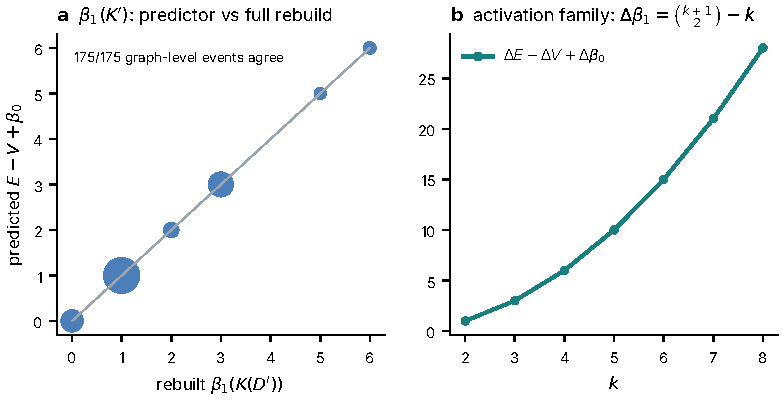
\includegraphics[width=\textwidth]{fig21_graph_update}
\caption{\textbf{Graph-level prediction (exact theorem; finite-exact test on $175$ events).} (a) Predicted $\beta_1(K')=E-V+\beta_0$ versus $\beta_1$ of the rebuilt complex, for the $175$ census events in which neither complex has $2$-cells (point size grows with multiplicity; all points lie on the diagonal). (b) $\Delta\beta_1=\binom{k+1}2-k$ for the activation family: the values for $k=2,\dots,5$ were recomputed, the points for $k=6,7,8$ are values of the proved formula, not computations.}\label{fig:graphupdate}
\end{figure}
\begin{counter}[a pierced edge with an increase of $\beta_1$ in the abstract calculus]\label{cx:abstract}
Take (as abstract sets) $D=\{56,21,32,45\}$ and $N=\{51,15,11\}$. Then $K(D)$ has edges $\{21,45\},\{21,56\},\{32,56\}$, $\beta=(1,0)$; $K(D\cup N)$ has $7$ vertices, $6$ edges, no $2$-cells and $\beta=(2,1)$; the edge $\{21,45\}$ is pierced (by $15\in[3,315]^\circ$) and $\beta_1$ nevertheless increases. This is a computation with the rule of \cref{thm:A5T31} and does not assert that such an event occurs along a collective orbit.
\end{counter}
\begin{remark}[a census regularity, not a theorem]
In the census below, the $251$ events with a dead edge never raise $\beta_1$. This regularity is not a law of the transition calculus (\cref{cx:abstract}); whether it can fail along a collective orbit is open.
\end{remark}

\subsection{Event types}
Every occurrence event adds at least one vertex. Classify an event $D\to D'$ by its effect on $(K,\beta)$:
\begin{center}\small
\begin{tabular}{@{}cl@{}}\toprule
Type & definition\\\midrule
I & the complex does not change\\
II & some $\beta_i$ increases and none decreases\\
III & some $\beta_i$ decreases and none increases\\
IV & some $\beta_i$ increases and some decreases\\
V & the Betti vector is unchanged while the complex changes\\\bottomrule
\end{tabular}
\end{center}
\begin{theorem}[no event of Type I; census]\label{thm:A5T7}
(a) Type I never occurs among occurrence events: $D\subsetneq D'$ adds a vertex, so $K\ne K'$. Hence every activation without a change of Betti numbers is of Type V.
(b) \emph{Census} (finite-exact, recomputed): for the orbits $x_0=S^2/\ell$ with $L(x_0)=S$, $G(x_0)=\ell$, $\ell\in\{5,7,11,13\}$, $S<1500$, followed for $24$ steps ($382$ orbits), the $2{,}576$ occurrence events are of Type V in $1{,}787$ cases, II in $603$, III in $172$, IV in $14$ and I in none. $251$ events have a dead edge (at most $16$ in one event) and $2{,}325$ are nested ($\mathrm{Dead}=\emptyset$); $\beta_2$ changes in $246$ events and $\beta_3$ in one; $\beta_1$ decreases in $176$ and increases in $388$. In each event the structural statements of \cref{thm:A5T32}, the zig-zag identity, the reconstruction of $\beta(K)$ and $\beta(K')$ from $(r,h,\beta(K^\circ))$, the local Euler formula and the cause criteria of \cref{thm:cause} hold (no exception).
(c) Table of the dependence of $\Delta\beta_1$ on the cause, ``dead edge?'' and ``new $2$-cell?'': (no,no): $178$ up, $27$ same, $0$ down; (no,yes): $210$, $1865$, $45$; (yes,no): $0$, $2$, $0$; (yes,yes): $0$, $118$, $131$. The empty ``down'' entry of (no,no) is \cref{thm:cause}; the zeros in the ``up'' column of both dead-edge rows are a census regularity (see above).
\end{theorem}
\prov{CW-0452}{A5-T7}{MIXED}{SPLIT}
\begin{proof}
(a) is the definition. (b), (c) are computations with the engine of Appendix~\ref{app:definitions}; the proved parts are those named. \qedhere
\end{proof}
\begin{remark}[no predictive predicate for the type]
What is proved is the \emph{form} of the answer: the type is determined by $(K(D),N)$, and $N$ is arithmetic (\cref{cor:event}). No arithmetic predicate of the state alone is claimed to predict the type; that is an open problem (\cref{sec:concl}). The inherited cross-check, that all $474$ step-activation events of the source census have the same Betti vectors before and after under this engine, is \stat{cited}.
\end{remark}
The distribution of event types is shown in \cref{fig:types}.
\begin{figure}[tbp]\centering
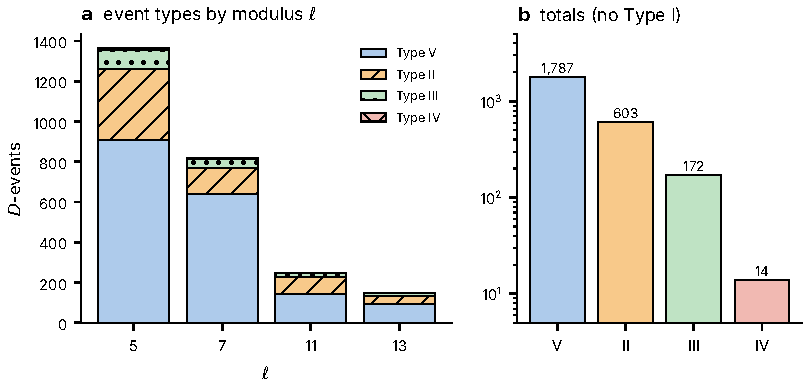
\includegraphics[width=\textwidth]{fig22_event_types}
\caption{\textbf{Event types in the census (finite-exact; $2{,}576$ events, $382$ orbits $x_0=S^2/\ell$ with $L=S$, $G=\ell$; $\ell=5,7,11,13$, $S<1500$, $24$ steps).} (a) Counts of Types V, II, III, IV for each $\ell$ (Type I is absent). (b) Totals $1{,}787$, $603$, $172$, $14$ on a log scale. The census is a finite sample drawn from a fixed parameter box and is not extrapolated.}\label{fig:types}
\end{figure}
